% Options for packages loaded elsewhere
\PassOptionsToPackage{unicode}{hyperref}
\PassOptionsToPackage{hyphens}{url}
\PassOptionsToPackage{space}{xeCJK}
%
\documentclass[
  a4paper,
  UTF8,
  fontset=none,
  zihao=5]{ctexart}
\usepackage{amsmath,amssymb}
\usepackage{iftex}
\ifPDFTeX
  \usepackage[T1]{fontenc}
  \usepackage[utf8]{inputenc}
  \usepackage{textcomp} % provide euro and other symbols
\else % if luatex or xetex
  \usepackage{unicode-math} % this also loads fontspec
  \defaultfontfeatures{Scale=MatchLowercase}
  \defaultfontfeatures[\rmfamily]{Ligatures=TeX,Scale=1}
\fi
\usepackage{lmodern}
\ifPDFTeX\else
  % xetex/luatex font selection
  \setmainfont[]{Latin Modern Roman}
  \ifXeTeX
    \usepackage{xeCJK}
    \setCJKmainfont[]{Noto Serif CJK SC}
          \setCJKsansfont[]{Noto Sans CJK SC}
              \setCJKmonofont[]{Noto Sans Mono CJK SC}
      \fi
  \ifLuaTeX
    \usepackage[]{luatexja-fontspec}
    \setmainjfont[]{Noto Serif CJK SC}
  \fi
\fi
% Use upquote if available, for straight quotes in verbatim environments
\IfFileExists{upquote.sty}{\usepackage{upquote}}{}
\IfFileExists{microtype.sty}{% use microtype if available
  \usepackage[]{microtype}
  \UseMicrotypeSet[protrusion]{basicmath} % disable protrusion for tt fonts
}{}
\makeatletter
\@ifundefined{KOMAClassName}{% if non-KOMA class
  \IfFileExists{parskip.sty}{%
    \usepackage{parskip}
  }{% else
    \setlength{\parindent}{0pt}
    \setlength{\parskip}{6pt plus 2pt minus 1pt}}
}{% if KOMA class
  \KOMAoptions{parskip=half}}
\makeatother
\usepackage{xcolor}
\usepackage[margin=23mm]{geometry}
\usepackage{longtable,booktabs,array}
\usepackage{calc} % for calculating minipage widths
% Correct order of tables after \paragraph or \subparagraph
\usepackage{etoolbox}
\makeatletter
\patchcmd\longtable{\par}{\if@noskipsec\mbox{}\fi\par}{}{}
\makeatother
% Allow footnotes in longtable head/foot
\IfFileExists{footnotehyper.sty}{\usepackage{footnotehyper}}{\usepackage{footnote}}
\makesavenoteenv{longtable}
\usepackage{graphicx}
\makeatletter
\def\maxwidth{\ifdim\Gin@nat@width>\linewidth\linewidth\else\Gin@nat@width\fi}
\def\maxheight{\ifdim\Gin@nat@height>\textheight\textheight\else\Gin@nat@height\fi}
\makeatother
% Scale images if necessary, so that they will not overflow the page
% margins by default, and it is still possible to overwrite the defaults
% using explicit options in \includegraphics[width, height, ...]{}
\setkeys{Gin}{width=\maxwidth,height=\maxheight,keepaspectratio}
% Set default figure placement to htbp
\makeatletter
\def\fps@figure{htbp}
\makeatother
\setlength{\emergencystretch}{3em} % prevent overfull lines
\providecommand{\tightlist}{%
  \setlength{\itemsep}{0pt}\setlength{\parskip}{0pt}}
\setcounter{secnumdepth}{5}
% definitions for citeproc citations
\NewDocumentCommand\citeproctext{}{}
\NewDocumentCommand\citeproc{mm}{%
  \begingroup\def\citeproctext{#2}\cite{#1}\endgroup}
\makeatletter
 % allow citations to break across lines
 \let\@cite@ofmt\@firstofone
 % avoid brackets around text for \cite:
 \def\@biblabel#1{}
 \def\@cite#1#2{{#1\if@tempswa , #2\fi}}
\makeatother
\newlength{\cslhangindent}
\setlength{\cslhangindent}{1.5em}
\newlength{\csllabelwidth}
\setlength{\csllabelwidth}{3em}
\newenvironment{CSLReferences}[2] % #1 hanging-indent, #2 entry-spacing
 {\begin{list}{}{%
  \setlength{\itemindent}{0pt}
  \setlength{\leftmargin}{0pt}
  \setlength{\parsep}{0pt}
  % turn on hanging indent if param 1 is 1
  \ifodd #1
   \setlength{\leftmargin}{\cslhangindent}
   \setlength{\itemindent}{-1\cslhangindent}
  \fi
  % set entry spacing
  \setlength{\itemsep}{#2\baselineskip}}}
 {\end{list}}
\usepackage{calc}
\newcommand{\CSLBlock}[1]{\hfill\break\parbox[t]{\linewidth}{\strut\ignorespaces#1\strut}}
\newcommand{\CSLLeftMargin}[1]{\parbox[t]{\csllabelwidth}{\strut#1\strut}}
\newcommand{\CSLRightInline}[1]{\parbox[t]{\linewidth - \csllabelwidth}{\strut#1\strut}}
\newcommand{\CSLIndent}[1]{\hspace{\cslhangindent}#1}
\ifLuaTeX
\usepackage[bidi=basic]{babel}
\else
\usepackage[bidi=default]{babel}
\fi
\babelprovide[main,import]{american}
\ifPDFTeX
\else
\babelfont{rm}[]{Latin Modern Roman}
\fi
% get rid of language-specific shorthands (see #6817):
\let\LanguageShortHands\languageshorthands
\def\languageshorthands#1{}
\usepackage{caption,etoolbox,setspace,fancyhdr}
\setstretch{1.17}
\setlength{\parindent}{2em}
\setlength{\parskip}{0.24em}
\setlength{\emergencystretch}{3em}
\setlength{\LTpre}{0.7em}
\setlength{\LTpost}{0.7em}
\AtBeginEnvironment{longtable}{\small\setlength{\tabcolsep}{4pt}}
\captionsetup{font=small,labelformat=empty}
\ctexset{
  section={name={,},number={\arabic{section}},format=\large\bfseries,
           beforeskip=1.25em,afterskip=.55em},
  subsection={format=\normalsize\bfseries,beforeskip=1em,afterskip=.35em}
}
\pagestyle{fancy}
\fancyhf{}
\fancyhead[C]{\small 面向大语言模型服务的推测解码综述}
\fancyfoot[C]{\thepage}
\renewcommand{\headrulewidth}{0.3pt}
\AtBeginDocument{\hypersetup{hidelinks,pdflang={zh-CN}}}
\ifLuaTeX
  \usepackage{selnolig}  % disable illegal ligatures
\fi
\usepackage{bookmark}
\IfFileExists{xurl.sty}{\usepackage{xurl}}{} % add URL line breaks if available
\urlstyle{same}
\hypersetup{
  pdftitle={面向大语言模型服务的推测解码综述},
  pdflang={en-US},
  hidelinks,
  pdfcreator={LaTeX via pandoc}}

\title{面向大语言模型服务的推测解码综述}
\usepackage{etoolbox}
\makeatletter
\providecommand{\subtitle}[1]{% add subtitle to \maketitle
  \apptocmd{\@title}{\par {\large #1 \par}}{}{}
}
\makeatother
\subtitle{Speculative Decoding for Large Language Model Serving: A
Survey}
\author{}
\date{}

\begin{document}
\maketitle

\subsection*{摘要}\label{abstract-zh}
\addcontentsline{toc}{subsection}{摘要}

推测解码以低成本候选换取目标模型并行验证，实际收益取决于一轮能提交多少有效输出、提交后的状态能否继续执行，以及推测新增工作如何影响同批请求。本文综述截至
2026 年 11 月 18
日的代表性研究和版本化实现，分别分析贪心一致、精确采样、合法前缀状态与服务收益的成立条件。通过比较检索与神经草稿、树形与块并行候选、验证预算和混合循环模型的状态恢复，本文说明，接受长度的改善只有在草稿、验证、恢复与调度的边际成本得到控制时才会降低单位输出代价。进一步以固定软件栈及可比评测为例，给出面向模型结构、负载和硬件的条件化研究问题。

\textbf{关键词：} 推测解码；大语言模型服务；精确采样；验证预算；前缀状态

\subsection*{Abstract}\label{abstract-en}
\addcontentsline{toc}{subsection}{Abstract}

Speculative decoding uses inexpensive proposals to expose parallel
verification in a target language model. Its practical benefit depends
on useful output per round, the validity of the state after commitment,
and the cost imposed on concurrent requests. This survey reviews
representative research and versioned implementations through November
18, 2026. It examines the conditions for greedy equivalence, exact
sampling, valid committed-prefix state, and serving gains. By comparing
retrieval and neural drafters, tree and block-parallel proposals,
verification budgets, and recurrent-state recovery in hybrid models, we
explain when longer acceptance translates into lower cost per emitted
token. Versioned software case studies and evidence comparisons ground
conditional research questions about model structure, workload, and
hardware.

\textbf{Keywords:} speculative decoding; large language model serving;
exact sampling; verification budget; committed-prefix state

\section{引言}\label{introduction}

自回归推理在位置 \(t\)
上必须等待前一输出确定，再从该前缀计算目标模型的条件分布。对于较小的在线批次，每新增一个
token
仍涉及目标权重访问、前缀状态读取和设备提交。推测解码先提供若干潜在后继，再将已知候选在目标模型中并行求值，从而让一轮有机会推进多个
token。Blockwise Parallel Decoding
用贪心前缀匹配刻画了这一机会，经典推测采样则通过拒绝与残差重采样保持目标抽样分布。两条路线共同依赖合法的因果前缀，却分别要求确定性一致与随机分布一致。{[}\citeproc{ref-blockwise}{1}--\citeproc{ref-chen}{3}{]}

在在线服务中，验证成本随批组成、上下文、并行布局和目标架构而变。一条候选比普通解码多处理若干位置，有时只增加少量时间，有时引起额外的缓存流量、专家执行与通信。即使一轮产生的
token
已经合法，目标与草稿侧还必须为下一轮构造与已提交前缀相符的状态。已有系统协同综述以草稿来源、候选几何、验证保真度和运行时执行组织工作，并将状态可实现性与端到端收益作为共同约束。Towards
Optimal Speculative Decoding
的公开摘要也将草稿效果、验证效率和系统执行联系起来。本文以这些已有综合为起点，将分析落实到一次可观察的提交、该提交对应的状态，以及同一负载下为它支付的关键路径成本。{[}\citeproc{ref-codesign}{4},\citeproc{ref-optimal}{5}{]}

本文给出三项综合。首先，以候选、验证和提交边界建立共同记号，说明随机验证与状态发布须满足哪些独立条件。其次，沿候选依赖、验证预算、状态恢复与执行路径比较代表机制，尤其关注块并行草稿与混合
GDN--MoE 目标的结合。最后，通过同基线证据对照解释离线吞吐、在线延迟和
SLO
指标的适用范围，并提出可用配对实验检验的研究问题。本文属于机制综合，所述性能测量来自相应一手来源。

第二节说明文献获取及已发表综述的覆盖。第三节建立共同记号，第四至第六节沿草稿、验证和运行时状态展开，第七节核对实验分母与基线，第八节给出可检验的后续问题。

\section{研究范围与文献获取}\label{scope}

本文采用问题导向的叙述性技术综述。研究截点为 2026 年 11 月 18
日，来源复核日期为 2026 年 11 月 18 日。以公开的 Decoding Acceleration
索引、11 月检索记录及网站既有专题索引定位候选，再以系统名、DOI、arXiv
编号和组合关键词追查原文，包括 ``speculative decoding recurrent
state''、``draft verification budget''、``MoE expert bytes'' 和
``hardware-aware speculative
decoding''。正文纳入直接改变候选、验证、提交状态或服务成本，并具有可定位方法或实现证据的工作。多模态结果用于解释条件信息和节点预算，泛
Agent
应用、非推测优化和缺乏可核查技术材料的候选不进入主论证。定向检索的覆盖范围随问题而定。{[}\citeproc{ref-awesome-index}{6},\citeproc{ref-website-index}{7}{]}

理论证明、作者实验、官方文档、固定源码和工程 PR
分别承担不同的论证职责。发表稿与同一成果的预印本按一个研究身份处理，参考条目标识实际使用的版本。对于
\emph{From Draft-Then-Verify to Systems Co-Design}，分类框架、方法剖面和
Co-Design Gates 依据公开 v1 全文，该版本形成 304 项研究的证据集，IEEE
发表摘要对应 312 项。\emph{Towards Optimal Speculative Decoding}
用于公开摘要层的研究定位，正式全文的目录、公式及评测细节未纳入本稿论证。{[}\citeproc{ref-codesign}{4},\citeproc{ref-optimal}{5},\citeproc{ref-codesign-ieee}{8}{]}

\section{正确性、前缀状态与单轮成本}\label{framework}

\subsection{一轮执行的观察边界}\label{round}

将一轮开始时已对外提交的 token 前缀记为 \(h\)。草稿提出长度 \(D\)
的候选链 \(y_{1:D}\)，或给出具备父指针的候选树。验证器对链中 \(K\)
个候选或树中 \(N\)
个候选节点求值。树中同层节点可能是互斥后继，实际输出只能沿一条从已提交前缀开始的合法路径。令
\(A\) 表示该轮接受的草稿 token 数，\(R\) 表示实际新增并提交的输出 token
数。全数接受时的 bonus token 或首次拒绝后的目标纠正 token 可能使
\(R=A+1\)。遇到
EOS、长度上限或取消时，按实际提交计数。实现也可能将本轮的最后一个新
token 留到下轮前向作为 anchor；应注明计算行是否含
anchor，避免将验证行数、草稿数和提交数混用。{[}\citeproc{ref-leviathan}{2},\citeproc{ref-chen}{3}{]}

\begin{longtable}[]{@{}
  >{\raggedright\arraybackslash}p{(\columnwidth - 4\tabcolsep) * \real{0.3333}}
  >{\raggedright\arraybackslash}p{(\columnwidth - 4\tabcolsep) * \real{0.3333}}
  >{\raggedright\arraybackslash}p{(\columnwidth - 4\tabcolsep) * \real{0.3333}}@{}}
\caption{表
1　单轮与批次的比较记号。时间以墙钟或明示的设备计时口径记录，长度以对应对象计数。}\tabularnewline
\toprule\noalign{}
\begin{minipage}[b]{\linewidth}\raggedright
记号
\end{minipage} & \begin{minipage}[b]{\linewidth}\raggedright
对象
\end{minipage} & \begin{minipage}[b]{\linewidth}\raggedright
含义
\end{minipage} \\
\midrule\noalign{}
\endfirsthead
\toprule\noalign{}
\begin{minipage}[b]{\linewidth}\raggedright
记号
\end{minipage} & \begin{minipage}[b]{\linewidth}\raggedright
对象
\end{minipage} & \begin{minipage}[b]{\linewidth}\raggedright
含义
\end{minipage} \\
\midrule\noalign{}
\endhead
\bottomrule\noalign{}
\endlastfoot
\(h,c,S_c\) & 提交与物化状态 & 逻辑前缀、已物化边界、该边界的执行状态 \\
\(D,K,N\) & 候选与预算 & 草稿链长、验证链长、树验证节点数 \\
\(A,R\) & 进度 & 接受的草稿数、实际提交的输出数 \\
\(B,L,Q\) & 执行形状 &
活跃解码请求数、上下文长度向量、实际目标查询行数 \\
\(T_0,T_{\mathrm{spec}}\) & 关键路径 & 同配置普通解码步与推测轮的时间 \\
\end{longtable}

在\hyperref[fig-round]{图
1}中，验证和输出提交沿同一逻辑路径，时间核算覆盖前后的执行及等待。

\begin{figure}
\centering
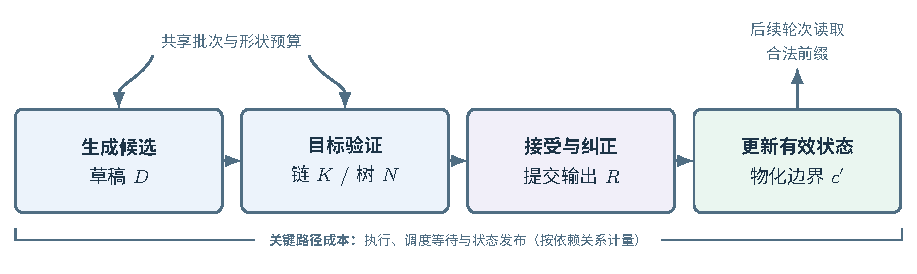
\includegraphics[width=1\textwidth,height=\textheight]{figures/specdec-round.pdf}
\caption{图 1　推测轮次、前缀状态与成本的关系。框中 \(D\)、\(K\)、\(N\)
与 \(R\) 的定义见表 1。箭头表示依赖与职责。}\label{fig-round}
\end{figure}

\subsection{验证规则决定保真度}\label{fidelity}

在给定相同 tokenizer、前缀、logits 变换和 tie-breaking
的数学模型下，贪心验证逐位置比较候选与目标
argmax，在第一个不匹配处由目标决定输出，沿因果路径归纳可得贪心一致。有限精度下，宽验证与逐
token 运行可能选择不同 kernel 或归约顺序。若目标的两个最高 logit
接近，微小差异也能改变 argmax。应分别说明数学保证与实测 token
一致率。放宽到 top-\(k\)
或以分数阈值直接接受，则改变了承诺，评估应回到任务质量或明确的近似准则。{[}\citeproc{ref-blockwise}{1},\citeproc{ref-chen}{3}{]}

精确的 token-wise
推测采样在每个已经沿草稿到达的位置使用两份条件分布。\(p_i(v)\)
是目标实际抽样分布，\(q_i(v)\) 是生成当前草稿 token
的真实分布，条件均为该位置的合法前缀，包含各自生效的温度、截断及其他变换。对
\(y_i\sim q_i\)，接受概率与首次拒绝的纠正分布分别为 \[
a_i(y_i)=\min\{1,p_i(y_i)/q_i(y_i)\},\qquad
r_i(v)=\frac{[p_i(v)-q_i(v)]_+}{\sum_u[p_i(u)-q_i(u)]_+}.
\]

接受的概率质量为 \(\min(p_i(v),q_i(v))\)，总拒绝质量为
\(\sum_u[p_i(u)-q_i(u)]_+\)，补回后恰得
\(p_i(v)\)。当分母为零时，该拒绝分支以概率零发生。所有候选被接受后，额外输出从下一位置的目标分布采样。跨位置的保证依赖条件分布与已提交前缀一致，因而同一随机种子下出现不同序列与分布正确性可以同时成立。树、多候选以及
block verification
各需核对自身的选择与纠正规则。{[}\citeproc{ref-leviathan}{2},\citeproc{ref-chen}{3}{]}

预算裁剪也有保真度前提。若在抽得本位置候选前按已知前缀和分数决定是否验证，经典规则可继续使用对应的条件
\(q_i\)。若选择依赖已经抽出的候选，验证器须匹配被选择对象的条件分布，或采用有独立证明的联合机制。以数学反例说明：令
\(p=q\) 为二元均匀分布，只在候选为 1 时用原 \(q\) 验证，否则从 \(p\)
重新采样。被验证的 1 总被接受，最终输出 1 的概率成为
\(3/4\)。这里产生偏差的原因是送去验证的候选已经改变分布。贪心前缀裁剪还有自己的一组条件，主要是目标计算的因果不变性、fallback
及状态重建。{[}\citeproc{ref-leviathan}{2},\citeproc{ref-codesign}{4}{]}

\subsection{合法前缀状态与发布}\label{state-invariant}

用 \(c\le |h|\) 表示目标实际物化到的位置，\(S_c\) 包括目标侧有效
KV、循环层及卷积状态，以及后续读取所需的索引和长度。对给定目标配置
\(\theta\)，状态契约要求 \[
S_c \simeq F_{\theta}(h_{1:c}),\qquad
\mathrm{pending}=h_{c+1:|h|}.
\] \(F_{\theta}\) 表示普通解码对该前缀的状态计算，\(\simeq\)
表示对后续目标计算可观察等价，有限精度时应给出容差或差分指标。物理块地址可以不同，逻辑位置、请求归属、有效范围和读写依赖必须相符。未提交分支可以暂存在设备缓冲中，但后续计算、其他请求及前缀缓存不可把它们当成合法历史。草稿缓存属于另一套状态，以其自身模型和同一合法历史重新裁剪、补齐或重建；它不需要与目标
KV 数值相等。{[}\citeproc{ref-codesign}{4}{]}

这一条件把验证与提交分开。验证器决定哪一段可以输出，提交器据此确定物化边界，必要时回收临时
KV、重建循环状态并发布计数。请求退出、槽位复用、异步 D2H
及图重放会引入额外的消费者排序要求。只检查当前轮返回的 token
可能放过被拒后缀残留到下一轮的问题。有限精度与状态污染也应分别定位，前者通常表现为相同逻辑前缀下的小幅计算差异，后者能通过先核对边界、索引和依赖再做差分来识别。{[}\citeproc{ref-codesign}{4}{]}

\subsection{从接受长度到单位有效输出时间}\label{cost}

对截断前的一条固定长度链，按 \(A\) 的尾和恒等式有
\(\mathbb{E}[A]=\sum_{j=1}^{K}\Pr(A\ge j)\)。其中每一项是前 \(j\)
个位置共同接受的概率，可以写成沿存活路径的条件概率连乘。常见比例模型以所有位置的条件接受概率相同为近似。请求类型、生成位置和已接受历史改变这些条件时，单个全局接受率无法准确恢复
\(\mathbb{E}[A]\)。同一平均接受率还可以对应不同的拒绝位置与落到关键路径上的恢复成本。{[}\citeproc{ref-leviathan}{2},\citeproc{ref-chen}{3}{]}

设一次执行依赖图中草稿、验证、选择、状态提交和运行时操作的持续时间分别由对应节点记录。串行时这些时间可以相加。存在并行准备、D2H
重叠或跨请求资源竞争时，用已测相互干扰条件下的关键路径时间
\(T_{\mathrm{spec}}\)，并把排队与调度间隙按测量范围单列。对串行、可比且可作长期统计的解码轮，单位输出代价及收益为
\[
g_{\mathrm{spec}}=\frac{\mathbb{E}[T_{\mathrm{spec}}]}{\mathbb{E}[R]},\qquad
g_0=\frac{\mathbb{E}[T_0]}{\mathbb{E}[R_0]},\qquad
\text{speedup}=\frac{g_0}{g_{\mathrm{spec}}} .
\]
这里用总时间除以总输出的相应估计量。计算批次吞吐时，应以所有请求的实际提交量之和作分子，共同的墙钟窗口只计一次。在线服务还应分别记录请求排队、首
token、token 间隔、完成分位数及 SLO
下的可持续请求率。离线单轮比值用于解释热路径，不能单独推导带到达过程的服务收益。{[}\citeproc{ref-codesign}{4},\citeproc{ref-optimal}{5}{]}

\section{候选生成与依赖结构}\label{drafting}

\subsection{从前缀检索到目标特征复用}\label{draft-sources}

候选来源首先决定草稿的固定开销与信息条件。独立小模型沿真实草稿历史逐
token 生成，自回归分解天然提供每个位置的条件 \(q_i\)。代价是额外权重、KV
和串行前向，轻载下这些成本可能被省下的目标步骤覆盖，高负载时草稿也会与目标争用设备。REST
从上下文末尾检索外部 datastore，以 trie
聚合延续，省去草稿模型训练与前向。其 §3 与 §4.3
表明，检索覆盖、语料匹配以及索引大小共同影响结果。运行时 prompt lookup
有类似的前缀匹配思想，但引用 REST 的实验不能为某个引擎的 n-gram
路径给出性能数字。候选来源的主要设定应是可用的上下文证据、构造成本及回退路径。{[}\citeproc{ref-leviathan}{2},\citeproc{ref-chen}{3},\citeproc{ref-rest}{9},\citeproc{ref-illusion}{10}{]}

目标集成式草稿复用主模型内部表征，代价转移到特征提取、读写和额外模块。Medusa
将若干未来位置的预测头接到目标模型，再把候选组合为树。Medusa-1 冻结
backbone，Medusa-2 联合微调，论文的 typical acceptance
另有质量评测边界。DeepSeek-V3 报告的 MTP 以逐深度模块训练后续 token
并保持因果链，训练目标可以用于改善基础模型，推理时也可把这些模块作为草稿。是否加载
MTP、保存哪些中间状态以及用何种验证器，由实际部署决定。多预测头输出与已部署的精确推测解码之间还隔着候选构造和验证契约。{[}\citeproc{ref-medusa}{11},\citeproc{ref-deepseek}{12}{]}

EAGLE 的核心是目标高层特征及已抽取的后继 token
共同给草稿提供条件，缓解下一层特征的多义性。EAGLE-2
根据上下文相关的草稿置信度动态选树，改变的是验证预算内的路径覆盖。EAGLE-3
转向直接 token
预测，融合多个深度的目标特征，并在训练阶段模拟推理时连续使用自身预测表示的过程。EAGLE-2
的树预算与 EAGLE-3
的训练和特征接口可以组合。对集成成本的比较须记录读取哪些层、是否增加跨设备搬运，以及拒绝后如何对齐草稿特征。用接受长度单独归因，容易把训练、采样和树选择的改变计给同一个组件。{[}\citeproc{ref-eagle}{13}--\citeproc{ref-eagle3}{15}{]}

\subsection{树的路径覆盖与块的生成并行性}\label{draft-geometry}

SpecInfer
将候选整理为前缀树，以祖先掩码和位置映射为每个节点计算正确的条件
logits。多个分支共享候选前缀，目标验证只沿被选路径提交，其他节点的暂态必须作废。其
§4.2--4.4
分别讨论树形目标求值及贪心/随机验证，树注意力只提供路径对应的目标分布，随机质量分配仍需对应的算法。相比相同最大深度的一条链，树可能降低早期误猜造成的整段浪费，同时会增加验证行数、掩码构造、缓存写入和树路径管理。树预算比较因此应同时报告深度、节点数及每个已提交
token
对应的实际目标行。{[}\citeproc{ref-codesign}{4},\citeproc{ref-eagle2}{14},\citeproc{ref-specinfer}{16}{]}

DFlash
在目标上下文特征的条件下用轻量块扩散草稿一次预测整个块，消除了完整 draft
backbone
的逐位置前向。其论文的块预测与目标验证提供了低草稿延迟的机制线索，精确语义仍须落实到部署采用的采样、纠正与状态更新。DSpark
在并行块 backbone 后增加轻量因果 head，使用前一 token 或循环状态修正草稿
logits，恢复块内条件信息，并加上置信估计来控制验证前缀。Domino
类似地将高成本 backbone
与轻量递归的因果修正分开，并通过分阶段训练协调两者。ChainFlow
将并行候选建模为目标特征条件下的少步潜变量流，加入 token
feedback，可生成链或树。比较的因果问题是：每增加一段因果条件，接受前缀增长是否覆盖串行
head、词表投影、重估和额外状态开销。{[}\citeproc{ref-dflash}{17}--\citeproc{ref-chainflow}{20}{]}

DDTree 把 DFlash
的位置级候选用固定节点预算编成树，增加分叉覆盖。位置分数沿分叉使用时，母路径已经变化，原来的位置边缘分布不再代表实际分支条件。DForkTree
用目标生成语料中的 n-gram PMI 修正分叉附近的候选排序，在 GPU
上构建树。其 Table 1 的主要对照共享草稿、目标验证器和 32
节点预算，但各方法使用在开发集选择的 proposal block
长度。该比较支持联合构树配置的收益，不能单独识别 PMI
在等块长上的贡献。D3Tree 以训练的节点存活 head
估计边际价值，按负载裁剪、匹配目标 GEMM
的形状预算。其多模态实验把视觉条件、模型结构和预算交织在一起，为负载下的几何选择提供证据，文本在线的收益范围仍需对应测量。{[}\citeproc{ref-ddtree}{21}--\citeproc{ref-d3tree}{23}{]}

\begin{longtable}[]{@{}
  >{\raggedright\arraybackslash}p{(\columnwidth - 4\tabcolsep) * \real{0.3333}}
  >{\raggedright\arraybackslash}p{(\columnwidth - 4\tabcolsep) * \real{0.3333}}
  >{\raggedright\arraybackslash}p{(\columnwidth - 4\tabcolsep) * \real{0.3333}}@{}}
\caption{表
2　候选生成机制与验证接口。几何描述提交给验证器的候选形状。}\tabularnewline
\toprule\noalign{}
\begin{minipage}[b]{\linewidth}\raggedright
代表方法
\end{minipage} & \begin{minipage}[b]{\linewidth}\raggedright
草稿条件及依赖
\end{minipage} & \begin{minipage}[b]{\linewidth}\raggedright
接口与主要开销
\end{minipage} \\
\midrule\noalign{}
\endfirsthead
\toprule\noalign{}
\begin{minipage}[b]{\linewidth}\raggedright
代表方法
\end{minipage} & \begin{minipage}[b]{\linewidth}\raggedright
草稿条件及依赖
\end{minipage} & \begin{minipage}[b]{\linewidth}\raggedright
接口与主要开销
\end{minipage} \\
\midrule\noalign{}
\endhead
\bottomrule\noalign{}
\endlastfoot
小模型推测采样 {[}\citeproc{ref-leviathan}{2},\citeproc{ref-chen}{3}{]}
& 独立草稿自回归，条件包含已抽样前缀 &
链和逐位置条件分布；草稿权重、串行步及 KV \\
REST {[}\citeproc{ref-rest}{9}{]} & 历史后缀检索与 trie 聚合 &
匹配候选路径；检索、索引容量及覆盖差异 \\
Medusa、MTP {[}\citeproc{ref-medusa}{11},\citeproc{ref-deepseek}{12}{]}
& 目标集成头；未来位置头或因果深度模块 &
多头候选或链；头的执行、训练与模型版本 \\
SpecInfer、EAGLE 系列
{[}\citeproc{ref-eagle}{13}--\citeproc{ref-specinfer}{16}{]} &
多草稿树、目标特征、置信选树 & 祖先掩码和位置；树
packing、暂态与提交映射 \\
DFlash、DSpark、Domino
{[}\citeproc{ref-dflash}{17}--\citeproc{ref-domino}{19}{]} & 并行
backbone；后两者加轻量因果修正 &
整块或前缀；块长、词表投影及轻量串行开销 \\
DDTree、DForkTree、D3Tree
{[}\citeproc{ref-ddtree}{21}--\citeproc{ref-d3tree}{23}{]} &
从位置候选构树，按分叉或存活信息重排 &
父闭合子树；形状、裁剪成本及路径状态 \\
\end{longtable}

接受目标本身也应与生成代价对齐。REAL Loss
以真实沿路径的接受长度为训练目标，指出用目标轨迹替代接受轨迹可能引入权重偏差。其
Qwen3.6-35B-A3B 和 Domino 的受控实验衡量接受长度的变化。EDR
进一步处理位置落在哪一轮的问题，以目标 rollouts
估计期望轮数。两者分别改善单轮接受目标与多轮计数目标，最终仍要考虑轮时变化，尤其是后缀长度、树形状或不同验证路径会改变目标工作量时。{[}\citeproc{ref-realloss}{24},\citeproc{ref-edr}{25}{]}

\section{目标验证与预算选择}\label{verification}

\subsection{从固定窗口到边际收益}\label{marginal-budget}

候选生成和目标验证可以使用不同预算。扩大链长或节点数一般增加覆盖机会，也把更多工作放入
\(Q\)，且 \(Q\) 到耗时的映射受图桶、tile、KV
长度和并行配置制约。对一个局部可比较的执行状态，令
\(G=\mathbb{E}[R]\)、\(C=\mathbb{E}[T]\)，新增候选后分别变化
\(\Delta G,\Delta C\)，并令
\(\lambda=G/C\)。当两种方案的时间都为正时，提高单位时间提交量等价于 \[
\Delta G > \lambda \Delta C .
\] 这只是两个配置的代数比较。\(\Delta G\)
需估计候选确实落入已提交路径的概率，\(\Delta C\)
应包含新增草稿、验证、发布与可见等待。在线队列还受分批边界和其他请求影响，因此该比较只为给定工作状态提供成本信号。块级拒绝采样也能提高同一候选块的
\(\mathbb{E}[R]\)。Sun 等在固定外层算法和合法验证器族中证明 block
verification
的进度最优性，并用相应纠正分布维持精确抽样。词表归约、设备支持和实际端到端成本仍属于额外证据。{[}\citeproc{ref-leviathan}{2},\citeproc{ref-blockverification}{26}--\citeproc{ref-sglangdocs}{28}{]}

MagicDec 说明高批量的费用曲线还取决于上下文。当长上下文推高 KV
读取，草稿通过稀疏 KV
降低自身费用，目标可在共享前缀读取中摊销验证行。短上下文与计算饱和情形可能出现不同趋势。\emph{Performance
or Illusion?} 在 vLLM 多模型、多负载、多个 draft
策略的测量中进一步量化了多区间的收益差异，指出验证经常占主导，接受长度也随任务与位置波动。它们共同支持按
\((B,L,Q)\)
测量，批量本身不足以确定验证是否昂贵。长上下文结论还需固定实际读写的缓存精度和生成长度。{[}\citeproc{ref-illusion}{10},\citeproc{ref-magicdec}{29}{]}

\subsection{批次、请求与两阶段预算}\label{batch-budget}

TableTune 在固定引擎上剖析不同批大小与长度的实际 step，生成批级
draft-length 表，再用在线接受计数纠偏。它强调切换长度会改变执行图和
pad，生产路径上的时延比孤立 kernel 推导更接近决策目标。DSpark 和 vLLM
Adaptive Verification
使用请求内的前缀存活分数，在全批范围分配验证位置。vLLM
当前文档将启动时的 shape 计时作为总量依据，将置信 head、可在线校准的
logit estimator 或 suffix
统计作为估计来源。后继位置只能随合法父前缀进入验证。采用抽样候选时，预算的每一步决策还须满足\hyperref[fidelity]{验证规则}所述条件。{[}\citeproc{ref-dspark}{18},\citeproc{ref-tabletune}{30},\citeproc{ref-avdocs}{31}{]}

即使验证已裁剪，并行草稿仍可能先生成完整块。ForeSpark 将预算分到 draft
前和 draft
后。前置估计利用目标上下文特征，按请求决定出草稿长度。后置整理利用生成后的信息分配目标验证行，同时用设备内排序和打包控制策略本身的关键路径。作者用同
backbone 的无联合调度变体隔离这部分收益，在 ShareGPT
定制引擎中同时报告匹配用户速率的总吞吐和开放到达下的 SLO 达成。Figure
8--9 还表明，在最重的 Qwen3-14B decode-only 负载里 AR
的吞吐仍居首，而在包含长历史和 prefill 的 ShareGPT-E2E
中排序发生变化。该对照说明应分别记录未生成、已生成未验证、已验证未提交三种工作，以及形状缩短是否真的减少设备时间。{[}\citeproc{ref-forespark}{32}{]}

预算也可以在部署级求解。SpecSearch
先用显存与成本约束剪去不可行配置，再对硬件校准并选择 AR
或推测、草稿长度与精度。其留出 GPU
的预测器以已有校准数据为基础，不能视作任意新后端都无需验证。与 TableTune
相比，它改变更外层的配置及内存条件。Hybrid Spark
研究另外一层分派，在代码编辑等有大量重复的内容上切换 n-gram 与
DSpark。部署选择、草稿来源选择与在线验证预算可串接，但需单独测量各自开销和切换时的状态对齐。{[}\citeproc{ref-tabletune}{30},\citeproc{ref-specsearch}{33},\citeproc{ref-hybridspark}{34}{]}

\subsection{混合 GDN--MoE 的阶段化验证}\label{hybrid-budget}

混合目标使每个新增验证位置的价格更不均匀。GDN 推进循环状态，MoE
的专家集合和路由分布改变权重访问、token--expert 并行度及可能的通信。Lan
的专家字节研究分辨按 slot 重复读与按专家并集读，分别测量 kernel
的带宽，说明仅用被激活专家数难以预测最优长度。其 §5
的理论边界包括几何接受、近似平稳路由、忽略草稿费用以及 batch-one
的硬件测量。可将每个 rank 的专家并集字节
\(U_r\)、分发负载及同步等待作为诊断特征，具体价格仍随实现变化。{[}\citeproc{ref-moebytes}{35}{]}

HybridSpec 先根据已校准的延迟和草稿置信选取窗口，在第一个 MoE router
之前额外计算一个候选位置。观察该候选给本层增加的专家后，再决定是否保留它进入余下目标前向。其目标是避免在全量专家执行后才决定是否支付扩展成本。第一个
router 的专家信息用于修正局部估计，后续层仍依赖校准或估计。原文附录 C.2
限定了因果前缀不变性、无会改变已保留前缀计算的容量限制、精确算术与状态恢复。附录
C.3 进一步给出点质量草稿的随机验证证明。对任何先验固定的候选 \(d_i\)，以
\(p_i(d_i)\) 接受，否则在排除 \(d_i\)
的目标分布中重采样。因为该规则在给定 \(d_i\) 时即复原 \(p_i\)，router
可以查看确定性草稿并裁剪，只要决定在本轮验证随机抽样前完成。一般随机草稿用原
\(q_i\)
直接做同样的裁剪并不享有这一证明。{[}\citeproc{ref-hybridspec}{27}{]}

\section{合法状态与服务运行时}\label{runtime}

\subsection{Transformer KV 与循环状态的提交粒度}\label{commit-state}

在标准因果注意力中，一个已知路径的每个位置有确定的 KV
和逻辑位置。拒绝后可以沿接受路径保留有效行、更新长度和映射，释放或遮蔽其他暂态。对树而言，选择路径与取得合法
KV
页是两个动作。采用分页缓存时，块内可能同时有合法和无效位置，页保留不能替代有效长度校验。跨请求复用或外部
KV connector 还应验证缓存身份由正确历史生成。SpecInfer
的树状态和前缀缓存给出了直接机制例子。Callo
则提供另一种边界：由上下文修改导致失效的旧 KV
可以用于提出候选，最终输出仍在新前缀的精确 KV 到位后验证。其收益还依赖
prefill--decode
分离中的渐进传输及排队，不能全部归因于推测。{[}\citeproc{ref-codesign}{4},\citeproc{ref-specinfer}{16},\citeproc{ref-callo}{36}{]}

循环层把一段历史压入共享状态。若在同一状态张量上顺序推进到被拒后缀，单纯缩小逻辑长度无法恢复接受边界。常用方案包括保留逐位置快照、从较早检查点重放、以及保留紧凑因子后重建。HybridSpec
将链验证的 GDN
更新改写为因果三角计算，把接受前缀所需的因子保留到提交，跨层一次写回接受状态，另需维护卷积和注意力缓存。Twig
在树上使用按祖先依赖的紧凑因子，选出路径后重建单个持久状态，并以批量目标延迟约束选节点预算。两者利用接受路径可压缩的结构，链的三角布局与树的祖先布局各有索引、临时内存与打包要求。全模型前向依旧存在层间依赖，跨层并行针对独立的提交重建。{[}\citeproc{ref-hybridspec}{27},\citeproc{ref-twig}{37}{]}

固定检查点的位置并非总要在输出刚提交时更新。vLLM 的 RecoverSSM 草案
\#66595 将提交后的接受计数留给下一次验证，由验证重放上一轮的已接受
token，并在请求离开 runner 时处理 pending
state。这使``逻辑输出已发布''和``状态已物化''成为明确的两个边界。如果调度器缓存或迁移请求，需保证读取到的检查点和待重放信息属于同一请求世代，且只对同一已提交历史重放一次。该例是截至复核时仍开放的代码提案，能说明协议选择，运行收益及通用兼容需独立确认。{[}\citeproc{ref-pr-recover}{38}{]}

\hyperref[fig-commit]{图
2}对比了目标侧两类状态的合法提交粒度。混合模型可以在同一轮使用两种路径。

\begin{figure}
\centering
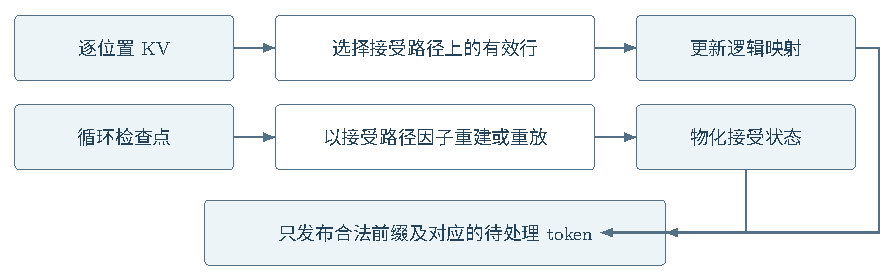
\includegraphics[width=1\textwidth,height=\textheight]{figures/state-commit.pdf}
\caption{图 2　注意力 KV
与循环检查点的提交。物理回收可由后端延后，后续消费者只读取合法的状态范围。}\label{fig-commit}
\end{figure}

\subsection{固定 vLLM 与 Ascend 路径}\label{fixed-runtime}

在 vLLM 固定提交
\texttt{0fc695fc6d1d82e9a5ac6835ac8e4e1c83703665}，调度器的
\texttt{schedule} 在 token
预算和请求进度下安排本轮工作，\texttt{update\_draft\_token\_ids}
接收候选。GPU MRV2 的 \texttt{BaseSpeculator.propose}
接收批次、目标隐藏特征、接受或拒绝计数及抽样信息。Runner 的
\texttt{prepare\_inputs} 和 \texttt{execute\_model} 准备 token
行、位置和 KV block tables。目标 \texttt{sample} 在存在草稿时调用
\texttt{rejection\_sampler} 并传入 draft
logits，得到抽样与拒绝计数。\texttt{postprocess\_sampled} 首先通过
\texttt{post\_update} 更新 token、计算进度和请求统计，再调用
\texttt{model\_state.postprocess\_state}
处理模型专用状态。采样配置中还存在 synthetic
方法，调试模式产生的接受计数不提供分布保证。以上证据定位到 MRV2
的相关代码路径，整体功能入口以官方文档补充。{[}\citeproc{ref-vllm-pin}{39}--\citeproc{ref-vllmdocs}{43}{]}

vLLM-Ascend 固定 \texttt{5cb98caaadeff42b5b62b996e34bb2aaa29d20fd} 的
MRV2 在继承提交路径后增加一条 CPU
消费链。独立复制流等待当前生产者流，异步回传
\texttt{num\_computed\_tokens} 并记录
event。\texttt{\_update\_seq\_lens\_cpu}
在读取已缓存请求对应的槽位前同步该 event，再加上本轮调度的 token 数形成
CPU 长度元数据。这表明，D2H
字节数虽小，消费者能否提前继续仍由等待集决定。后续 \#21430
提议将复制发起移到设备状态提交之前，保留上一计数写入的依赖，并主张新请求写槽与旧请求
CPU
消费槽可以分开。该排序的可移植条件是生产者、消费者和槽位的真实依赖成立，不能只根据调用位置提早就判定正确。{[}\citeproc{ref-ascend-pin}{44},\citeproc{ref-pr-d2h}{45}{]}

图重放降低潜在的提交开销，能覆盖到哪一步取决于
shape、资源寿命、拷贝及后端支持。vLLM \#63421 把 adaptive verification
的预算选择替换为预热的一次 Triton
launch，改的是调度开销和编译停顿。Ascend \#19512 的 DFlash2 Full
ACLGraph 覆盖 MRV2 下的草稿前向、候选选择和草稿缓存更新，其作者评测对应
Qwen3.8-27B-W8A8、4×910B4 与 TP4。\#20254 仍在评审，针对 rejection
sampling 的 host launch 和图重放，特殊采样路径仍有
fallback。这些版本各自落在决策、草稿或采样热路径，具体可组合性须按目标模型、量化、图模式及硬件检查。旧版
pair 的静态证据不回答这些更新在 910B2
上是否通过。{[}\citeproc{ref-pr-av}{46}--\citeproc{ref-ascenddocs}{49}{]}

\subsection{共享资源与端到端瓶颈}\label{serving-cost}

草稿优化的收益受它在关键路径上的占比约束。Weights That Stay 把 serial
head 的词表投影分片驻留在 on-chip 存储上，在单个 persistent kernel
中推进状态和选择 token，减少重复访存及 host launch。该论文在单 H100 的
SGLang Qwen3-4B/8B Markov 草稿集成中分别报告最高 12.3\%/8.6\%
的客户端吞吐提升，B200
的头部容量实验处在另一测量层。能否迁移取决于投影分片、片上可用容量、同步以及目标计算与草稿资源干扰。优化草稿缓存也有类似的分母问题。Gupta
与 Li 在 Qwen2.5-3B/1.5B 的 batch-one 原型里测得 packed K4V4
减少草稿缓存存储字节，Table 8 的整体峰值分配却与对应 BF16
推测设置相同，1K 与 16K 的端到端平均时延均更长。该表的 batched verifier
还出现 greedy token
与顺序参考不一致，应保留这项数值边界。{[}\citeproc{ref-weights}{50},\citeproc{ref-draftkv}{51}{]}

服务资源按共享窗口消费。草稿权重、额外 KV
页、循环状态、保留多个形状的图缓冲和大 batch 的 padding
会改变可同时容纳的请求数。每请求 TPOT 下降可能伴随更少的可用 KV 页或更高
TTFT。当 decode 与 chunked prefill 共享目标
step，增加一条候选可能延长当前 prefill 等待，并通过排队放大后续请求的
tail latency。SGLang
文档的例子也说明，随机验证模式与链宽、硬件后端和分离部署相关。在 SGLang
固定 DFlash runner 中，\texttt{\_chain\_accept\_indices}
生成接受行索引，目标状态有独立的
\texttt{\_update\_target\_mamba\_state\_after\_verify}
路径。固定实现还会在部分设备缺乏非贪心验证时产生贪心 fallback
提示，明确指出请求分布无法保持。应用最新文档选项时须再查部署版本。{[}\citeproc{ref-illusion}{10},\citeproc{ref-sglangdocs}{28},\citeproc{ref-forespark}{32},\citeproc{ref-sglang-pin}{52}{]}

\section{实验证据的可比性}\label{evidence}

\subsection{对齐分母与匹配基线}\label{comparison}

至少要区分草稿 acceptance
rate、每轮接受草稿数、每轮实际提交量、每次目标调用的查询行数和服务输出
token/s。HybridSpec 的 AL 和 DForkTree 的 \(\tau\) 含目标补发的
token，草稿训练论文的接受长度可能不含它。ForeSpark
把内部预算优化讨论中的 goodput 用于有效接受工作，实际开放服务另报告
TTFT、TPOT 同时达标的请求比例和达到 90\% 达标时的到达率。论文使用
goodput 一词时应复述其定义。闭环固定并发、开环固定请求率和离线固定 batch
对客户端等待与重填有不同控制，须各自比较。{[}\citeproc{ref-illusion}{10},\citeproc{ref-dforktree}{22},\citeproc{ref-hybridspec}{27},\citeproc{ref-forespark}{32}{]}

同一结论的最强基线取决于消融对象。要问草稿是否更好，应匹配
target、verifier、候选预算和采样；要问验证策略是否有效，应共享 drafter
并匹配状态提交、图覆盖和内存；要问端到端是否更快，应记录原生
AR、固定推测和强自适应三个可用参照，同时允许极端负载回到
AR。不同硬件、量化、TP/EP、模型、请求轨迹、prompt/output
长度、前缀缓存和 graph
设置会破坏直接比较。推荐报告逐长度/负载区间的退化与失败，而非只保留单个最优点。{[}\citeproc{ref-illusion}{10},\citeproc{ref-tabletune}{30},\citeproc{ref-specsearch}{33}{]}

\begin{longtable}[]{@{}
  >{\raggedright\arraybackslash}p{(\columnwidth - 4\tabcolsep) * \real{0.3333}}
  >{\raggedright\arraybackslash}p{(\columnwidth - 4\tabcolsep) * \real{0.3333}}
  >{\raggedright\arraybackslash}p{(\columnwidth - 4\tabcolsep) * \real{0.3333}}@{}}
\caption{表
3　代表性作者实验与各自的证据边界。表中数字来自对应原文或对原表同条件数据的直接读取。}\tabularnewline
\toprule\noalign{}
\begin{minipage}[b]{\linewidth}\raggedright
工作与定位
\end{minipage} & \begin{minipage}[b]{\linewidth}\raggedright
对照条件
\end{minipage} & \begin{minipage}[b]{\linewidth}\raggedright
可支持的判断
\end{minipage} \\
\midrule\noalign{}
\endfirsthead
\toprule\noalign{}
\begin{minipage}[b]{\linewidth}\raggedright
工作与定位
\end{minipage} & \begin{minipage}[b]{\linewidth}\raggedright
对照条件
\end{minipage} & \begin{minipage}[b]{\linewidth}\raggedright
可支持的判断
\end{minipage} \\
\midrule\noalign{}
\endhead
\bottomrule\noalign{}
\endlastfoot
HybridSpec Table 1、Appendix E {[}\citeproc{ref-hybridspec}{27}{]} &
SGLang 0.5.16、A100 80 GB、三个 Qwen3.5/3.6 GDN--MoE 与官方
DFlash，SPEED-Bench 主表 280 测试请求，单请求贪心 & 按类别汇总的
post-prefill speedup 为 AR 的 1.75--1.88 倍。附录另有温度 1
两组模型与四并发闭环，覆盖有限 \\
ForeSpark Figures 8--9 {[}\citeproc{ref-forespark}{32}{]} & vLLM
0.30.0，Qwen3-14B TP8 H100；GLM 系列 TP8+EP8
B200。ShareGPT，主结果为贪心 & Qwen3-14B 在 ShareGPT-E2E
开放到达下，90\% 达标时的请求率为 DSpark 的 1.51 倍，为最强基线的 1.20
倍 \\
TableTune Table 1、§6 {[}\citeproc{ref-tabletune}{30}{]} & H100，vLLM
V2，闭环模型及草稿组合，对照逐负载最佳固定长度 &
五组测试中四组的校准表达到最佳固定基线吞吐的至少
94\%。图模式影响表的可转移性 \\
Twig §§VI--VII {[}\citeproc{ref-twig}{37}{]} & SGLang，A100/GB10，含
Qwen3.5 和混合模型的树验证；有离线和 Open-SWE-Traces 在线案例 & 分开测树
verifier、整模型与在线尾部时延。收益依赖状态
kernel、预算和端到端调度组合 \\
SpecSearch Figure 2、§V {[}\citeproc{ref-specsearch}{33}{]} &
Qwen3-4B、RTX 5090，vLLM AR 与 DFlash 配置，短输出、不同并发 & 在该
sweep 中 DFlash 吞吐由并发 2 的 AR 3.50 倍变成并发 64 的 0.76
倍。设备与内存校准决定排序 \\
Draft KV quantization Table 8 {[}\citeproc{ref-draftkv}{51}{]} &
Qwen2.5-3B/1.5B，1K/16K、256 输出、batch one，packed K4V4 与 BF16 SD &
实际缓存字节下降与整体峰值不变、解码变慢同时出现。该原型不等于生产在线服务 \\
\end{longtable}

HybridSpec 的 Table 1 和 Table 3 给出一个直接的反例：Qwen3.6-35B-A3B
的主表平均提交量从 vanilla DFlash 的 4.79 降至 4.57，平均 AR
归一化速度却从 1.37 增至
1.83。这里的收益来自少验证与更高效的循环状态处理的组合。与此同时，附录
E.7 的同模型四客户端运行，整体吞吐只比 vanilla DFlash 高约
10\%，批中请求共用一个窗口长度。对比两者应保留负载、基线和分母，避免把单请求加速推广到服务
SLO。{[}\citeproc{ref-hybridspec}{27}{]}

\subsection{11 月增量证据的处理}\label{november}

采用首次提交和所用版本两个时间字段可避免把修订当成新工作。HybridSpec、DForkTree、D3Tree、ForeSpark、REAL
Loss、ChainFlow 和 SpecSearch 作为 11 月新预印本参与相应机制论证。Twig
从 8 月首投更新到 11 月 v2，Weights That Stay 首投为 10 月 31 日、列入
11 月序号。ForeSpark 引用 11 月 13 日 v2，DForkTree 与 D3Tree
分别用于分叉分数与负载裁剪。两者的文本与多模态评测各自保留。此次还追查了
Callo、草稿 KV 量化、Hybrid Spark 及 SpecPilot。SpecPilot
对推测优化的部署依赖提供交叉证据，但其复合搜索同时改变目标权重格式、树验证与批处理等因素，本文只用来说明配置依赖，并将可归因的主比较建立在匹配消融上。{[}\citeproc{ref-chainflow}{20},\citeproc{ref-dforktree}{22}--\citeproc{ref-realloss}{24},\citeproc{ref-hybridspec}{27},\citeproc{ref-forespark}{32}--\citeproc{ref-hybridspark}{34},\citeproc{ref-callo}{36},\citeproc{ref-twig}{37},\citeproc{ref-weights}{50},\citeproc{ref-draftkv}{51},\citeproc{ref-specpilot}{53}{]}

\section{开放问题与可检验研究方向}\label{directions}

\subsection{状态恢复何时应立即发生}\label{deferred-commit}

HybridSpec 已把链式重建跨层合并，Twig 已在树上将接受路径压紧，RecoverSSM
提案给出延迟重放的直接设计。进一步的研究问题是：在连续批处理、请求退出、prefix-cache
发布和图/eager
交替的共同边界上，何时能把恢复延迟到下一次消费者，何时必须把接受状态立即物化。假设是把检查点、接受路径和请求世代作为共同约束，可以在同样状态内存预算下减少前台等待。可用立即重建、检查点重放和部署已支持的延迟重放作基线，固定已提交
token 轨迹并注入首位拒绝、末位拒绝、全收、结束与 slot
复用。核对下一轮真实
logits、状态索引、重放计数和消费者事件。如果恢复最终总被严格串到相同消费者之前，或者额外的
pending
状态抵消节省，假设即失效。{[}\citeproc{ref-hybridspec}{27},\citeproc{ref-twig}{37},\citeproc{ref-pr-recover}{38},\citeproc{ref-pr-d2h}{45}{]}

\subsection{路由与资源信息能否改进批内选择}\label{routing-aware-scheduling}

DSpark、ForeSpark 和 TableTune
已覆盖置信、批级实测和联合预算。HybridSpec 则利用第一个 router
的实际专家信息，专家字节研究给出 kernel 复用解释。值得验证的是在 TP/EP
下，分位 rank 的路由负载、专家并集以及通信是否提供超过 shape
成本表的增量信息。应在同一对
drafter/target、相同图候选与内存预算内先测最强固定
\(K\)、按形状的自适应预算与联合预算，再增加 router
特征。报告估计误差、控制开销、实际 all-to-all
等待和每轮有效输出。分别做只解码、混合 prefill、KV
长短及请求偏斜的测试。若通信或 graph
切换吞掉可省时间，或真实专家负载可由 shape
表充分解释，则保留更简单策略。Ascend
的候选实验需先确认目标、drafter、精度、图模式和 TP
组合的可运行性。{[}\citeproc{ref-dspark}{18},\citeproc{ref-hybridspec}{27},\citeproc{ref-tabletune}{30},\citeproc{ref-forespark}{32},\citeproc{ref-moebytes}{35}{]}

\subsection{训练目标能否对应服务效用}\label{training-to-serving}

REAL Loss 建模路径接受，EDR 建模到完成需要的轮数，ForeSpark
则处理实测服务资源分配。它们自然引出一个配对问题：当服务控制器能按负载选择
\(D,K\)
或回退，增加较深位置的接受概率是否还改善服务指标。实验可冻结同一个目标模型、部署实现和训练资源，比较
token 似然、EAL、EDR
与按已测边际成本加权的训练目标。先做同条件的存活曲线与数值一致性，再在多负载下做真实时间、草稿费用和
SLO
达成的配对测量，并测试在新上下文分布和目标内核下的排序是否稳定。若改善集中在从未获准验证的位置、或通过增加串行
draft
计算获得，服务收益可能消失。对于任何数据依赖的随机预算，应按实际验证机制复核目标抽样分布。{[}\citeproc{ref-codesign}{4},\citeproc{ref-realloss}{24},\citeproc{ref-edr}{25},\citeproc{ref-forespark}{32}{]}

\section{结论}\label{conclusion}

推测执行的收益来自用可承受的新增工作换取更多合法提交。贪心一致由目标
argmax
与因果条件决定，精确随机验证还需匹配提议、选择和纠正分布。一次合法输出须对应能继续运行的前缀状态，尤其在树形候选、循环层、图重放和异步服务中，缓存位置、请求所有权和发布顺序共同决定下一轮是否有效。

草稿、验证和状态优化的相对价值随目标结构、上下文、设备和负载而变。块并行减轻草稿前向后，瓶颈可以移到验证和状态恢复；负载变重后，控制候选和请求间分配的收益还会被形状、缓存容量及调度开销约束。由此，机制比较应将实际提交量与关键路径配对，并把固定源码、作者实验、线上
SLO 与硬件迁移放回各自的适用条件。

\section*{参考文献}\label{references}
\addcontentsline{toc}{section}{参考文献}

\phantomsection\label{refs}
\begin{CSLReferences}{0}{0}
\bibitem[\citeproctext]{ref-blockwise}
\CSLLeftMargin{{[}1{]} }%
\CSLRightInline{M. Stern, N. Shazeer, and J. Uszkoreit. Blockwise
parallel decoding for deep autoregressive models. Advances in neural
information processing systems, 2018.
\url{https://arxiv.org/abs/1811.03115v1}. Methods and evaluation read in
arXiv v1, first submitted 2018-11-07, reviewed 2026-11-18.}

\bibitem[\citeproctext]{ref-leviathan}
\CSLLeftMargin{{[}2{]} }%
\CSLRightInline{Y. Leviathan, M. Kalman, and Y. Matias. Fast inference
from transformers via speculative decoding. Proceedings of the 40th
international conference on machine learning, 2023, 202, 19274--19286.
\url{https://proceedings.mlr.press/v202/leviathan23a.html}. Published
full text reviewed 2026-11-18; first preprint arXiv:2211.17192,
submitted 2022-11-30.}

\bibitem[\citeproctext]{ref-chen}
\CSLLeftMargin{{[}3{]} }%
\CSLRightInline{C. Chen, S. Borgeaud, G. Irving, et al. Accelerating
large language model decoding with speculative sampling. 2023.
\url{https://arxiv.org/abs/2302.01318v1}. arXiv v1, first submitted
2023-02-02, reviewed 2026-11-18.}

\bibitem[\citeproctext]{ref-codesign}
\CSLLeftMargin{{[}4{]} }%
\CSLRightInline{K. Zhao, Z. Liu, C. Jiang, et al. From draft-then-verify
to systems co-design: A survey of speculative decoding for
autoregressive large language models. 2026.
\url{https://doi.org/10.20944/preprints202608.0746.v1}. Preprints.org
v1, submitted 2026-08-10, posted 2026-08-11, full text reviewed
2026-11-18.}

\bibitem[\citeproctext]{ref-optimal}
\CSLLeftMargin{{[}5{]} }%
\CSLRightInline{Y. Ji, W. Xu, X. Qian, et al. Towards optimal
speculative decoding: A comprehensive survey on optimizations and future
directions. ACM Computing Surveys, 2026, 59, (1).
\url{https://doi.org/10.1145/3846171}. Bibliographic record and public
abstract reviewed 2026-11-18.}

\bibitem[\citeproctext]{ref-awesome-index}
\CSLLeftMargin{{[}6{]} }%
\CSLRightInline{Awesome LLM Inference Systems. {Decoding Acceleration
and November 14 Literature Sweep}. 2026.
\url{https://github.com/sad-and-bad1231/awesome-LLM-inference-systems/blob/c12fd42879527f95e3f12bfbae5d2ef209aa4e3c/topics/decoding-acceleration.md}.
Discovery index and reviews/NOVEMBER\_2026\_DECODING\_SWEEP\_20261114.md
at the same revision; reviewed 2026-11-18.}

\bibitem[\citeproctext]{ref-website-index}
\CSLLeftMargin{{[}7{]} }%
\CSLRightInline{IntelliStream. {Speculative Decoding: Living Topic and
Frozen Report}. 2026.
\url{https://github.com/intellistream/auto-research-report-website/blob/b830bc4d74b3c2928e9f0c900c04c4b476555ebc/topics/speculative-decoding/survey.json}.
Discovery index only; revision b830bc4 includes the source and evidence
ledgers and the implementation audit; reviewed 2026-11-18.}

\bibitem[\citeproctext]{ref-codesign-ieee}
\CSLLeftMargin{{[}8{]} }%
\CSLRightInline{K. Zhao, Z. Liu, C. Jiang, et al. From draft-then-verify
to systems co-design: A survey of speculative decoding for
autoregressive large language models. IEEE Access, 2026, 14,
153987--154013. \url{https://doi.org/10.1109/ACCESS.2026.3739598}.
Published 2026-10-06; bibliographic record and abstract reviewed
2026-11-18, same study as preprint.}

\bibitem[\citeproctext]{ref-rest}
\CSLLeftMargin{{[}9{]} }%
\CSLRightInline{Z. He, Z. Zhong, T. Cai, et al. {REST: Retrieval-Based
Speculative Decoding}. NAACL 2024, 2024.
\url{https://arxiv.org/abs/2311.08252v2}. 2311.08252v2, first submitted
2023-11-14, cited revision 2024-04-04; §§3--4 reviewed 2026-11-18.}

\bibitem[\citeproctext]{ref-illusion}
\CSLLeftMargin{{[}10{]} }%
\CSLRightInline{X. Liu, J. Yu, J. Park, et al. {Speculative Decoding:
Performance or Illusion?} 2025.
\url{https://arxiv.org/abs/2601.11580v2}. 2601.11580v2, first submitted
2025-12-31, cited revision 2026-03-18; experimental setup, verifier
profile and throughput reviewed 2026-11-18.}

\bibitem[\citeproctext]{ref-medusa}
\CSLLeftMargin{{[}11{]} }%
\CSLRightInline{T. Cai, Y. Li, Z. Geng, et al. {Medusa: Simple LLM
Inference Acceleration Framework with Multiple Decoding Heads}. ICML
2024, 2024. \url{https://arxiv.org/abs/2401.10774v3}. 2401.10774v3,
first submitted 2024-01-19, cited revision 2024-06-14; §§2--3 reviewed
2026-11-18.}

\bibitem[\citeproctext]{ref-deepseek}
\CSLLeftMargin{{[}12{]} }%
\CSLRightInline{DeepSeek-AI, A. Liu, B. Feng, et al. {DeepSeek-V3
Technical Report}. 2024. \url{https://arxiv.org/abs/2412.19437v1}.
2412.19437v1, first submitted 2024-12-27; technical report §2.2 reviewed
2026-11-18.}

\bibitem[\citeproctext]{ref-eagle}
\CSLLeftMargin{{[}13{]} }%
\CSLRightInline{Y. Li, F. Wei, C. Zhang, and H. Zhang. {EAGLE:
Speculative Sampling Requires Rethinking Feature Uncertainty}. ICML
2024, 2024. \url{https://proceedings.mlr.press/v235/li24bt.html}.
2401.15077v1, first submitted 2024-01-26; §§3--5 reviewed 2026-11-18.}

\bibitem[\citeproctext]{ref-eagle2}
\CSLLeftMargin{{[}14{]} }%
\CSLRightInline{Y. Li, F. Wei, C. Zhang, and H. Zhang. {EAGLE-2: Faster
Inference of Language Models with Dynamic Draft Trees}. EMNLP 2024,
2024. \url{https://aclanthology.org/2024.emnlp-main.422/}. 2406.16858v1,
first submitted 2024-06-24, published full text used; tree construction
and evaluation reviewed 2026-11-18.}

\bibitem[\citeproctext]{ref-eagle3}
\CSLLeftMargin{{[}15{]} }%
\CSLRightInline{Y. Li, F. Wei, C. Zhang, and H. Zhang. {EAGLE-3: Scaling
up Inference Acceleration of Large Language Models via Training-Time
Test}. NeurIPS 2025, 2025.
\url{https://proceedings.neurips.cc/paper_files/paper/2025/hash/c7b5a35ea98b62512a869c19ea7b03cb-Abstract-Conference.html}.
2503.01840v1, first submitted 2025-03-03, published full text used;
training-time test and inference reviewed 2026-11-18.}

\bibitem[\citeproctext]{ref-specinfer}
\CSLLeftMargin{{[}16{]} }%
\CSLRightInline{X. Miao, G. Oliaro, Z. Zhang, et al. {SpecInfer:
Accelerating Generative Large Language Model Serving with Tree-based
Speculative Inference and Verification}. ASPLOS 2024, 2024.
\url{https://arxiv.org/abs/2305.09781v4}. 2305.09781v4, first submitted
2023-05-16, cited revision 2024-04-01; §4 and evaluation reviewed
2026-11-18.}

\bibitem[\citeproctext]{ref-dflash}
\CSLLeftMargin{{[}17{]} }%
\CSLRightInline{J. Chen, Y. Liang, and Z. Liu. {DFlash: Block Diffusion
for Flash Speculative Decoding}. 2026.
\url{https://arxiv.org/abs/2602.06036v2}. 2602.06036v2, first submitted
2026-02-05, cited revision 2026-05-28; method and evaluation reviewed
2026-11-18.}

\bibitem[\citeproctext]{ref-dspark}
\CSLLeftMargin{{[}18{]} }%
\CSLRightInline{X. Cheng, X. Yu, C. Shao, et al. {DSpark:
Confidence-Scheduled Speculative Decoding with Semi-Autoregressive
Generation}. 2026. \url{https://arxiv.org/abs/2607.05147v1}.
2607.05147v1, first submitted 2026-07-06; §§3.1--3.2 and serving
evaluation reviewed 2026-11-18.}

\bibitem[\citeproctext]{ref-domino}
\CSLLeftMargin{{[}19{]} }%
\CSLRightInline{J. Huang, Y. Zhang, Q. Zhang, et al. {Domino: Decoupling
Causal Modeling from Autoregressive Drafting in Speculative Decoding}.
Proceedings of the 2026 conference on empirical methods in natural
language processing, 2026, 23346--23356.
\url{https://doi.org/10.18653/2026.emnlp-main.1015}. Published §3 and
evaluation reviewed 2026-11-18.}

\bibitem[\citeproctext]{ref-chainflow}
\CSLLeftMargin{{[}20{]} }%
\CSLRightInline{S. Aktas, Y. E. Erdem, A. Zeer, et al. {ChainFlow:
Few-Step Latent Flow Matching for Speculative Decoding}. 2026.
\url{https://arxiv.org/abs/2611.08669v1}. 2611.08669v1, first submitted
2026-11-05; §§3--4 reviewed 2026-11-18.}

\bibitem[\citeproctext]{ref-ddtree}
\CSLLeftMargin{{[}21{]} }%
\CSLRightInline{L. Ringel and Y. Romano. {Accelerating Speculative
Decoding with Block Diffusion Draft Trees}. 2026.
\url{https://arxiv.org/abs/2604.12989v1}. 2604.12989v1, first submitted
2026-04-14; tree construction and evaluation reviewed 2026-11-18.}

\bibitem[\citeproctext]{ref-dforktree}
\CSLLeftMargin{{[}22{]} }%
\CSLRightInline{Z. Zheng, C. Zhang, and C. Tang. {DForkTree:
Accelerating Speculative Decoding with Fork-Aware Block Diffusion Draft
Trees}. 2026. \url{https://arxiv.org/abs/2611.12356v1}. 2611.12356v1,
first submitted 2026-11-09; §§3--5 and Table 1 reviewed 2026-11-18.}

\bibitem[\citeproctext]{ref-d3tree}
\CSLLeftMargin{{[}23{]} }%
\CSLRightInline{H. Nie, Z. Gao, J. Yu, et al. {D3Tree: Learning to Prune
Block-Diffusion Draft Trees for Efficient Verification}. 2026.
\url{https://arxiv.org/abs/2611.11371v1}. 2611.11371v1, first submitted
2026-11-08; node survival, runtime and Tables I--III reviewed
2026-11-18.}

\bibitem[\citeproctext]{ref-realloss}
\CSLLeftMargin{{[}24{]} }%
\CSLRightInline{Y. Tian. {REAL Loss: Optimizing Real Expected Acceptance
Length for Speculative Decoding}. 2026.
\url{https://arxiv.org/abs/2611.14399v1}. 2611.14399v1, first submitted
2026-11-10; training loss and controlled comparison reviewed
2026-11-18.}

\bibitem[\citeproctext]{ref-edr}
\CSLLeftMargin{{[}25{]} }%
\CSLRightInline{Y. Zhao and C. Cai. {Training Parallel Speculative Draft
Models by Directly Minimizing Expected Decoding Rounds}. 2026.
\url{https://arxiv.org/abs/2610.10411v1}. 2610.10411v1, first submitted
2026-10-07; Markov reward model and experiment reviewed 2026-11-18.}

\bibitem[\citeproctext]{ref-blockverification}
\CSLLeftMargin{{[}26{]} }%
\CSLRightInline{Z. Sun, U. Mendlovic, Y. Leviathan, et al. Block
verification accelerates speculative decoding. ICLR 2025, 2025.
\url{https://arxiv.org/abs/2403.10444v3}. First submitted 2024-03-15,
author proceedings version v3 dated 2025-04-10; Algorithms 1--3 and
Theorems 1--2 reviewed 2026-11-18.}

\bibitem[\citeproctext]{ref-hybridspec}
\CSLLeftMargin{{[}27{]} }%
\CSLRightInline{H. Wang, S. Q. Zhang, Z. Liu, and S. Li. {HybridSpec:
Throughput-Aware Speculative Decoding for Hybrid GDN-MoE Models}. 2026.
\url{https://arxiv.org/abs/2611.04055v1}. 2611.04055v1, first submitted
2026-11-02; §§3--4 and Appendices C--E reviewed 2026-11-18.}

\bibitem[\citeproctext]{ref-sglangdocs}
\CSLLeftMargin{{[}28{]} }%
\CSLRightInline{SGLang Project. {Speculative Decoding}. 2026.
\url{https://docs.sglang.io/docs/advanced_features/speculative_decoding}.
Live documentation, chain rejection and block verification constraints;
reviewed 2026-11-18.}

\bibitem[\citeproctext]{ref-magicdec}
\CSLLeftMargin{{[}29{]} }%
\CSLRightInline{R. Sadhukhan, J. Chen, Z. Chen, et al. {MagicDec:
Breaking the Latency-Throughput Tradeoff for Long Context Generation
with Speculative Decoding}. ICLR 2025, 2025.
\url{https://proceedings.iclr.cc/paper_files/paper/2025/hash/13f972adf12bdf886583d48cd528002f-Abstract-Conference.html}.
First submitted 2024-08-20 as arXiv:2408.11049; proceedings full text
reviewed 2026-11-18.}

\bibitem[\citeproctext]{ref-tabletune}
\CSLLeftMargin{{[}30{]} }%
\CSLRightInline{A. Malvankar, P. Castro, N. Mitchell, and L. Villard.
{TableTune: Measured, Self-Correcting Draft-Length Tables for Dynamic
Speculative Decoding}. 2026. \url{https://arxiv.org/abs/2610.38968v1}.
2610.38968v1, first submitted 2026-10-28; §§4, 6 and Table 1 reviewed
2026-11-18.}

\bibitem[\citeproctext]{ref-avdocs}
\CSLLeftMargin{{[}31{]} }%
\CSLRightInline{vLLM Project. {Adaptive Verification}. 2026.
\url{https://docs.vllm.ai/en/latest/features/speculative_decoding/adaptive_verification/}.
Live documentation, shape profiling and estimator support; reviewed
2026-11-18.}

\bibitem[\citeproctext]{ref-forespark}
\CSLLeftMargin{{[}32{]} }%
\CSLRightInline{J. Song, D. Wang, P. Patel, et al. {ForeSpark: Joint
Draft and Verification Budget Scheduling for Parallel Speculative
Decoding}. 2026. \url{https://arxiv.org/abs/2611.13442v2}. 2611.13442v2,
first submitted 2026-11-10, cited revision 2026-11-13; §§4--6, Figures
8--9, and Appendix C reviewed 2026-11-18.}

\bibitem[\citeproctext]{ref-specsearch}
\CSLLeftMargin{{[}33{]} }%
\CSLRightInline{S. Yildirim, A. Zeyrek, and D. Chen. {SpecSearch:
Towards Hardware-Aware Efficient Speculative Decoding}. 2026.
\url{https://arxiv.org/abs/2611.22296v1}. 2611.22296v1, first submitted
2026-11-17; §§III--V and Figure 2 reviewed 2026-11-18.}

\bibitem[\citeproctext]{ref-hybridspark}
\CSLLeftMargin{{[}34{]} }%
\CSLRightInline{E. Ranjan and B. Venkitesh. {Hybrid Spark: Adaptive
Speculative Decoding That Lets the Content Choose the Drafter}. 2026.
\url{https://arxiv.org/abs/2611.05611v1}. 2611.05611v1, first submitted
2026-11-03; drafter selection and vLLM evaluation reviewed 2026-11-18.}

\bibitem[\citeproctext]{ref-moebytes}
\CSLLeftMargin{{[}35{]} }%
\CSLRightInline{Y. Lan. {Speculative Decoding for Mixture-of-Experts
Models: Expert Bytes, Kernel Bandwidth and the Best Draft Length}. 2026.
\url{https://arxiv.org/abs/2610.34440v1}. 2610.34440v1, first submitted
2026-10-25; §§2--5, expert kernels and model limits reviewed
2026-11-18.}

\bibitem[\citeproctext]{ref-callo}
\CSLLeftMargin{{[}36{]} }%
\CSLRightInline{J. Ou and M. Lentz. {Callo: Serving Cache-Miss Requests
with Speculative Decoding on Invalidated KV under Prefill-Decode
Disaggregation}. 2026. \url{https://arxiv.org/abs/2611.18459v1}.
2611.18459v1, first submitted 2026-11-13; §§3--5, especially Table 3 and
streaming ablation reviewed 2026-11-18.}

\bibitem[\citeproctext]{ref-twig}
\CSLLeftMargin{{[}37{]} }%
\CSLRightInline{L. Wang, Y. Su, X. Wu, et al. {Twig: Parallel and
Memory-Efficient Tree Speculative Decoding for Hybrid-Attention LLMs}.
2026. \url{https://arxiv.org/abs/2608.01651v2}. 2608.01651v2, first
submitted 2026-08-03, cited revision 2026-11-05; §§IV--VII,
accepted-path state and serving protocols reviewed 2026-11-18.}

\bibitem[\citeproctext]{ref-pr-recover}
\CSLLeftMargin{{[}38{]} }%
\CSLRightInline{vLLM Project. {RecoverSSM: Replay the Accepted Tokens in
the Next Verify}. 2026.
\url{https://github.com/vllm-project/vllm/pull/66595}. Open draft PR at
cdced7fb9741c8eca9661c56883ea9828b90fcd3; reviewed 2026-11-18.}

\bibitem[\citeproctext]{ref-vllm-pin}
\CSLLeftMargin{{[}39{]} }%
\CSLRightInline{vLLM Project. {GPU Model Runner V2: Input Preparation,
Verification and State Commit}. 2026.
\url{https://github.com/vllm-project/vllm/blob/0fc695fc6d1d82e9a5ac6835ac8e4e1c83703665/vllm/v1/worker/gpu/model_runner.py\#L816}.
Pinned at 0fc695fc; prepare\_inputs, execute\_model, sample,
postprocess\_sampled; reviewed 2026-11-18.}

\bibitem[\citeproctext]{ref-vllm-scheduler}
\CSLLeftMargin{{[}40{]} }%
\CSLRightInline{vLLM Project. {V1 Scheduler: Speculative Token
Allocation and Draft Updates}. 2026.
\url{https://github.com/vllm-project/vllm/blob/0fc695fc6d1d82e9a5ac6835ac8e4e1c83703665/vllm/v1/core/sched/scheduler.py\#L340}.
Pinned at 0fc695fc; schedule and update\_draft\_token\_ids; reviewed
2026-11-18.}

\bibitem[\citeproctext]{ref-vllm-sampler}
\CSLLeftMargin{{[}41{]} }%
\CSLRightInline{vLLM Project. {GPU Rejection Sampler}. 2026.
\url{https://github.com/vllm-project/vllm/blob/0fc695fc6d1d82e9a5ac6835ac8e4e1c83703665/vllm/v1/worker/gpu/spec_decode/rejection_sampler.py\#L44}.
Pinned at 0fc695fc; sampling parameters, draft logits and synthetic
mode; reviewed 2026-11-18.}

\bibitem[\citeproctext]{ref-vllm-draft}
\CSLLeftMargin{{[}42{]} }%
\CSLRightInline{vLLM Project. {GPU BaseSpeculator Proposal Interface}.
2026.
\url{https://github.com/vllm-project/vllm/blob/0fc695fc6d1d82e9a5ac6835ac8e4e1c83703665/vllm/v1/worker/gpu/spec_decode/speculator.py\#L25}.
Pinned at 0fc695fc; BaseSpeculator.propose; reviewed 2026-11-18.}

\bibitem[\citeproctext]{ref-vllmdocs}
\CSLLeftMargin{{[}43{]} }%
\CSLRightInline{vLLM Project. {Speculative Decoding}. 2026.
\url{https://docs.vllm.ai/en/latest/features/speculative_decoding/}.
Live documentation; reviewed 2026-11-18.}

\bibitem[\citeproctext]{ref-ascend-pin}
\CSLLeftMargin{{[}44{]} }%
\CSLRightInline{vLLM-Ascend Project. {Ascend Model Runner V2: Counter
Publication and CPU Sequence Lengths}. 2026.
\url{https://github.com/vllm-project/vllm-ascend/blob/5cb98caaadeff42b5b62b996e34bb2aaa29d20fd/vllm_ascend/worker/v2/model_runner.py\#L388-L440}.
Pinned at 5cb98caa; state postprocess, D2H event, and CPU reader;
reviewed 2026-11-18.}

\bibitem[\citeproctext]{ref-pr-d2h}
\CSLLeftMargin{{[}45{]} }%
\CSLRightInline{vLLM-Ascend Project. {Issue the Computed-Token D2H
Snapshot before RecoverSSM Commit in MRV2}. 2026.
\url{https://github.com/vllm-project/vllm-ascend/pull/21430}. Open PR at
a0c28fd17a3bda74d3d2d5e431be28245b068ddf; reviewed 2026-11-18.}

\bibitem[\citeproctext]{ref-pr-av}
\CSLLeftMargin{{[}46{]} }%
\CSLRightInline{vLLM Project. {Replace Adaptive Verification Budget
Selection with a Triton Kernel}. 2026.
\url{https://github.com/vllm-project/vllm/pull/63421}. Merged 2026-10-26
at 41f5146b5b3a5b3c89ceee6f804e5e535a72ccbb; reviewed 2026-11-18.}

\bibitem[\citeproctext]{ref-pr-graph}
\CSLLeftMargin{{[}47{]} }%
\CSLRightInline{vLLM-Ascend Project. {Enable DFlash2 Full ACL Graph
Drafting on MRV2}. 2026.
\url{https://github.com/vllm-project/vllm-ascend/pull/19512}. Merged
2026-11-03 at 56af62b5159c0345db5e25ee7fb1623d4b327903; reviewed
2026-11-18.}

\bibitem[\citeproctext]{ref-pr-sampling}
\CSLLeftMargin{{[}48{]} }%
\CSLRightInline{vLLM-Ascend Project. {Replay Rejection Sampling Kernels
from One ACL Graph}. 2026.
\url{https://github.com/vllm-project/vllm-ascend/pull/20254}. Open PR at
fe58a4cf1c89190bffe5f43b8d7220bfb875d31a; reviewed 2026-11-18.}

\bibitem[\citeproctext]{ref-ascenddocs}
\CSLLeftMargin{{[}49{]} }%
\CSLRightInline{vLLM-Ascend Project. {Speculative Decoding}. 2026.
\url{https://docs.vllm.ai/projects/ascend/en/main/user_guide/feature_guide/speculative_decoding.html}.
Live documentation, proposer and backend configuration; reviewed
2026-11-18.}

\bibitem[\citeproctext]{ref-weights}
\CSLLeftMargin{{[}50{]} }%
\CSLRightInline{X. Qiang, Z. Xu, Z. Pan, et al. {Weights That Stay:
On-Chip Megakernels for Serial Heads in Speculative Decoding}. 2026.
\url{https://arxiv.org/abs/2611.00506v1}. 2611.00506v1, first submitted
2026-10-31; §§4--5, head benchmarks and system integration reviewed
2026-11-18.}

\bibitem[\citeproctext]{ref-draftkv}
\CSLLeftMargin{{[}51{]} }%
\CSLRightInline{S. Gupta and M. Li. {Memory-Efficient Speculative
Decoding with Quantized Draft KV Cache}. 2026.
\url{https://arxiv.org/abs/2611.20565v1}. 2611.20565v1, first submitted
2026-11-16; §§4--6 and Appendix E, Table 8 reviewed 2026-11-18.}

\bibitem[\citeproctext]{ref-sglang-pin}
\CSLLeftMargin{{[}52{]} }%
\CSLRightInline{SGLang Project. {DFlash Worker V2}. 2026.
\url{https://github.com/sgl-project/sglang/blob/f4c16239a557734690ff6652e392f36ac3788798/python/sglang/srt/speculative/dflash_worker_v2.py}.
Pinned at f4c16239a557734690ff6652e392f36ac3788798; accepted indices and
target recurrent-state update; reviewed 2026-11-18.}

\bibitem[\citeproctext]{ref-specpilot}
\CSLLeftMargin{{[}53{]} }%
\CSLRightInline{K. Li, W. Chai, Y. Liang, et al. {SpecPilot: Autonomous
Algorithm Discovery and Systems Optimization for Speculative Decoding}.
2026. \url{https://arxiv.org/abs/2611.02501v1}. 2611.02501v1, first
submitted 2026-11-02; multi-optimization design and evaluation reviewed
2026-11-18.}

\end{CSLReferences}

\end{document}
